% !TEX root = ../my-thesis.tex
%
\chapter{Results and timing analysis}
\label{sec:results}

\begin{figure*}[h]
    \centering
    \begin{subfigure}[b]{0.475\textwidth}
        \centering
        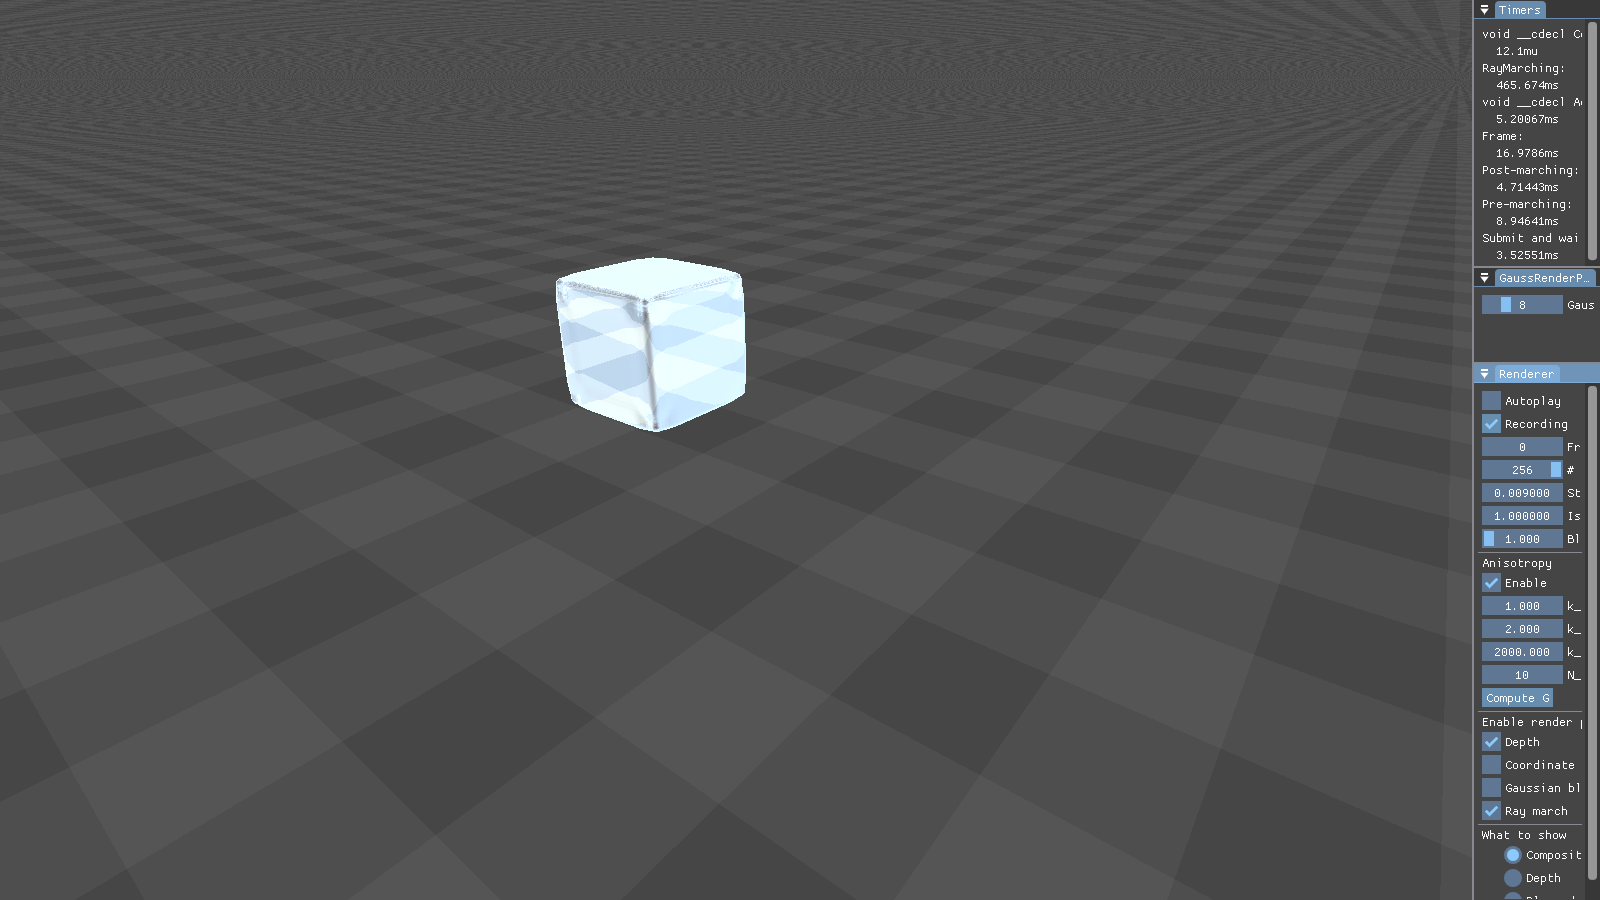
\includegraphics[width=\textwidth]{my-gfx/figure-result-1.png}  
    \end{subfigure}
    \hfill
    \begin{subfigure}[b]{0.475\textwidth}  
        \centering 
        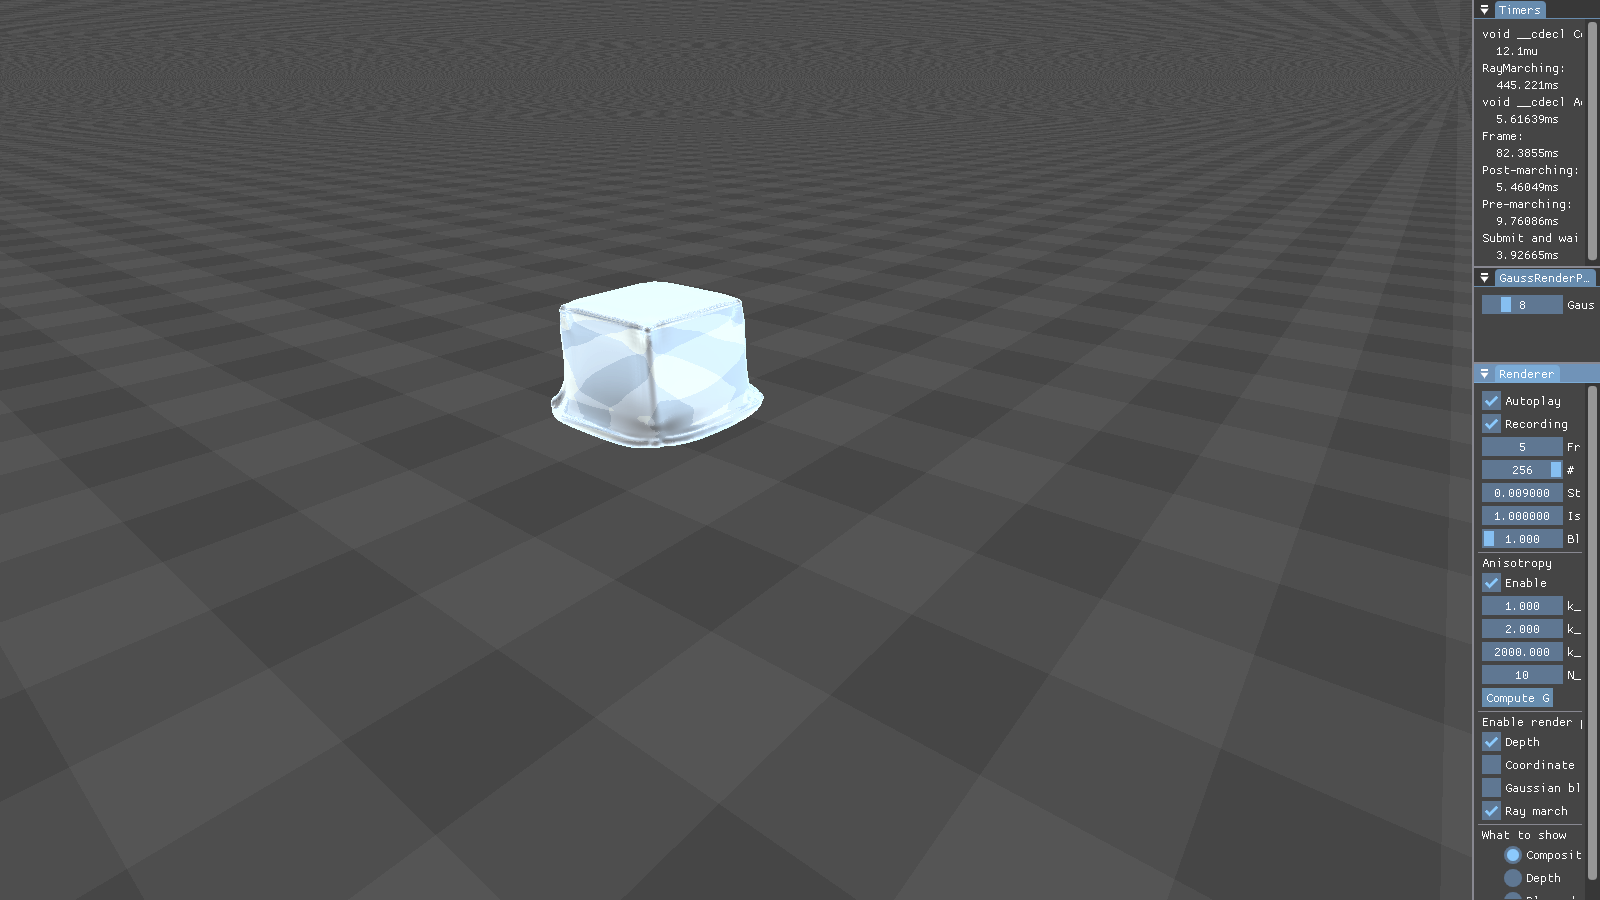
\includegraphics[width=\textwidth]{my-gfx/figure-result-2.png} 
    \end{subfigure}
    \vskip\baselineskip
    \begin{subfigure}[b]{0.475\textwidth}   
        \centering 
        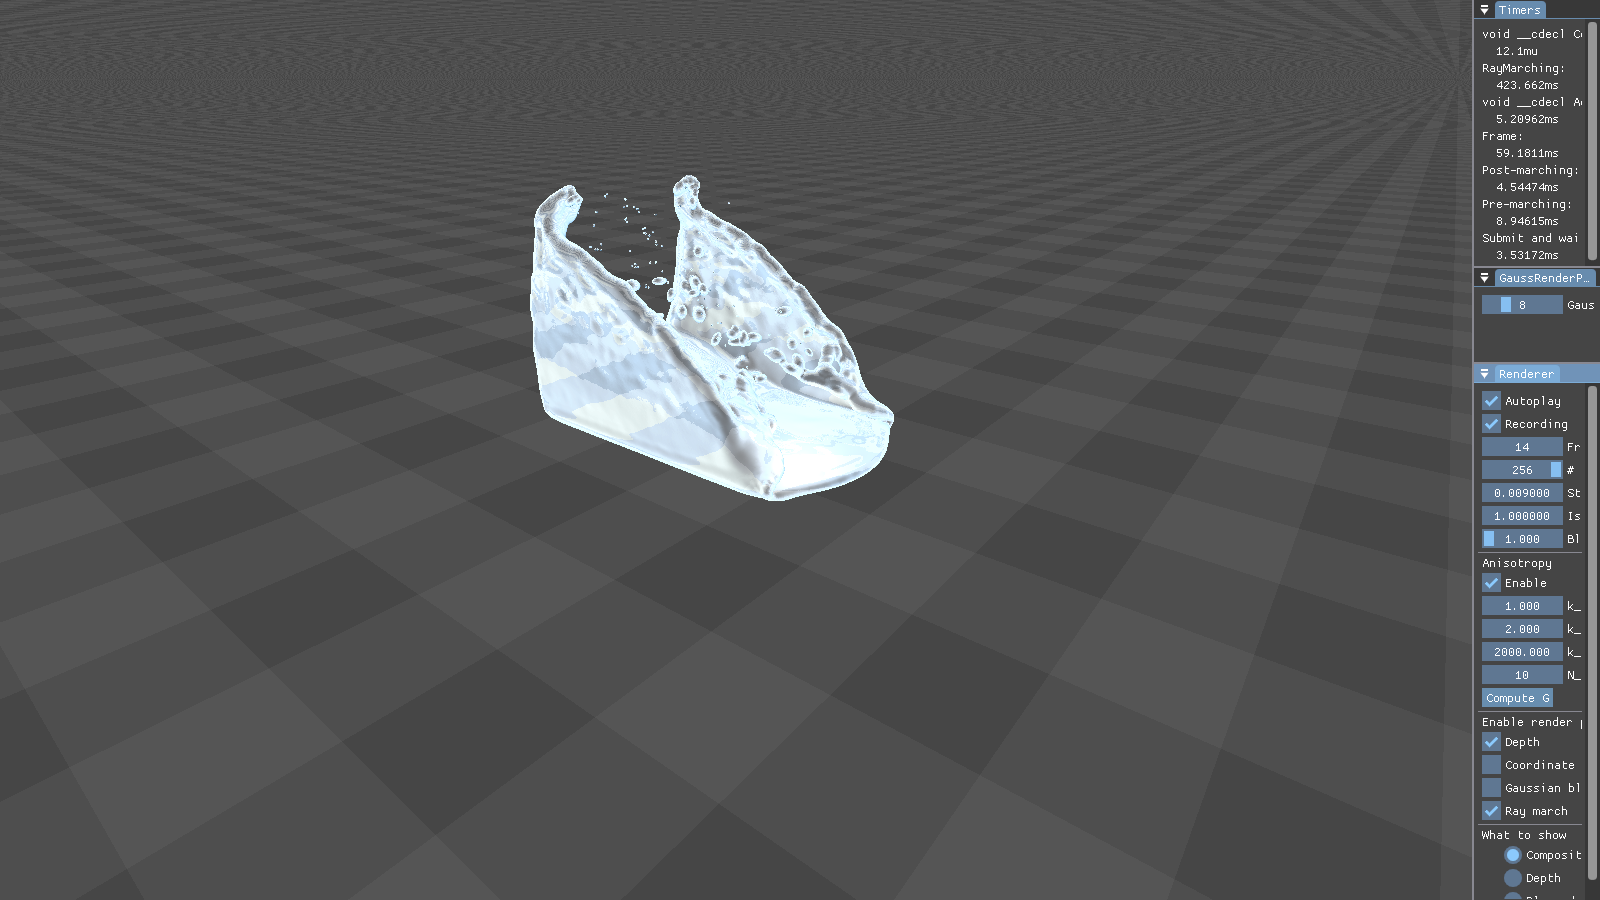
\includegraphics[width=\textwidth]{my-gfx/figure-result-3.png}  
    \end{subfigure}
    \hfill
    \begin{subfigure}[b]{0.475\textwidth}   
        \centering 
        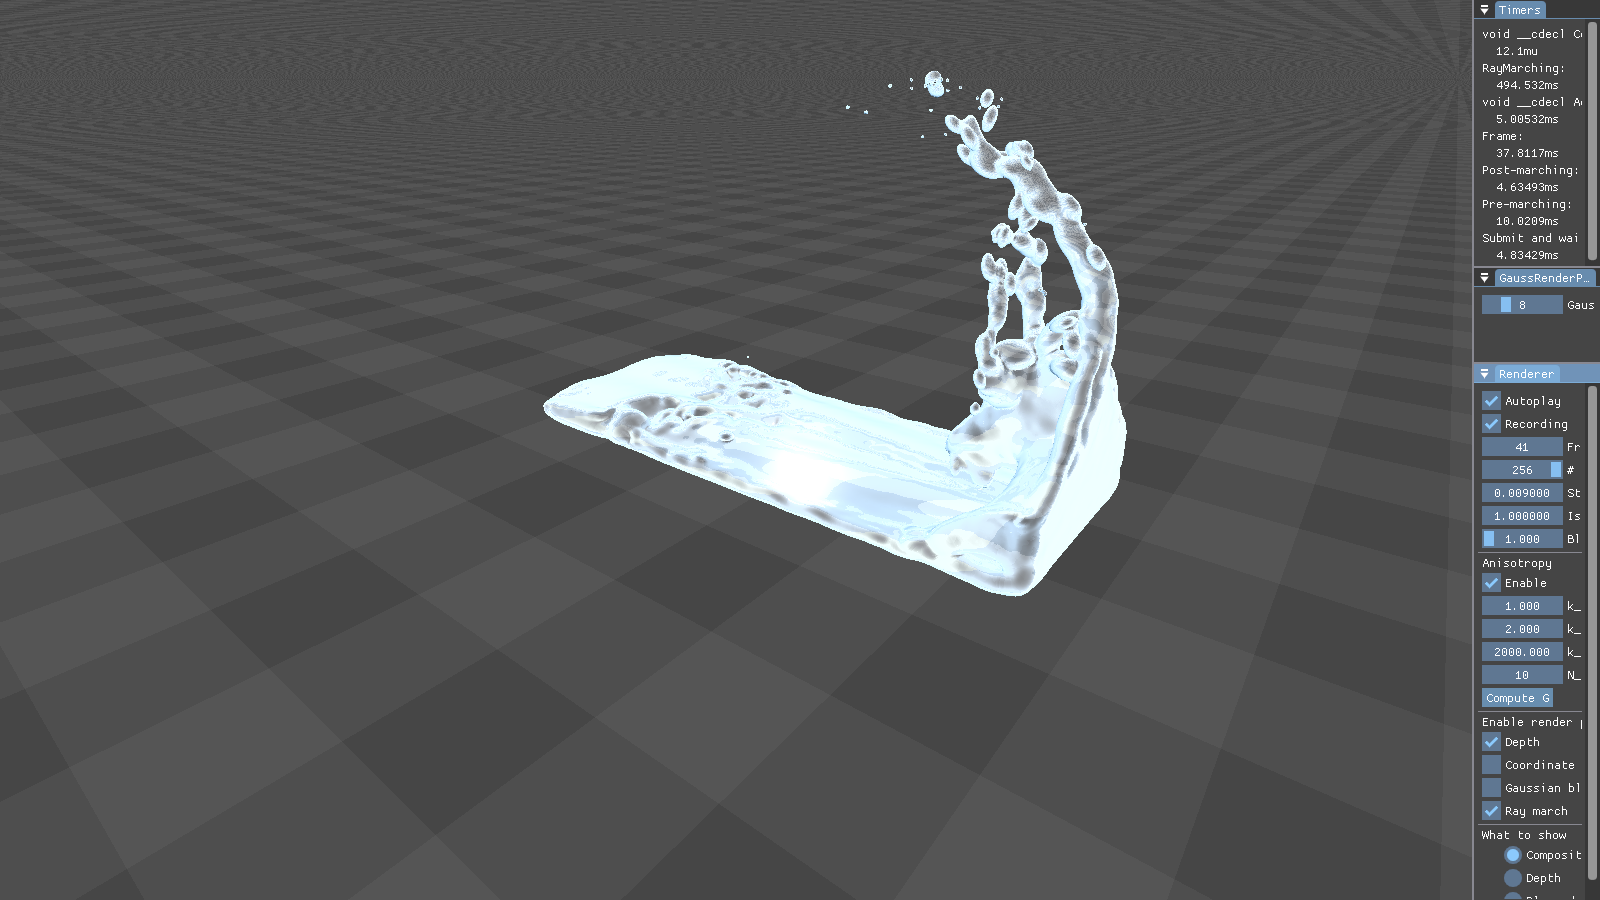
\includegraphics[width=\textwidth]{my-gfx/figure-result-4.png}
    \end{subfigure}
    
    \caption{Four snapshots of our visualization: A cube of fluid dropping into a box.}
    \label{fig:results}
\end{figure*}

Figure \myref{fig:results} shows the results our implementation can produce. Although the particles are spherical by nature, the flat faces of the initial cube configuration still appear to be flat. Particles close to each other merge into threads of fluid, creating a connected surface. Refraction, specularity, and a bluish tinge round off the illusion of water.

With many configurable parameters, the algorithm is very versatile and can be applied to all kinds of fluids. For example, Wu et al. show chocolate running down a model of a bunny in Figure 10 of their paper.

Timing tests were performed on a specific frame of the dam break dataset using a $1600 \times 900$ screen. The exact parameters like the camera position can be extracted from the code repository. The tests ran on an AMD Ryzen 7 1700X 8-core processor and an NVIDIA GeForce GTX 1060 graphics card. On average, the ray marching took $385\text{ms}$ with adaptive step lengths and $404\text{ms}$ with equal step lengths. For this specific scenario, a speedup of around $1.05$ was measured. Note that there are still significant improvements to be achieved when using the techniques Wu et al. propose.
